\chapter{切换到保护模式}\label{cha:latex-brief-intro}

\section{实验内容}
引导扇区突破 512 个字节的限制,将工作分给 loader;加载 loader 进入内存并运行;将控制权交给 loader。

\section{代码分析}

\subsection{核心数据结构}

% Please add the following required packages to your document preamble:
% \usepackage{multirow}
\begin{table}[htbp]
\begin{center}
\caption{boot.asm的主要数据结构}
\begin{tabular}{|c|l|l|}
\hline
\multirow{19}{*}{\begin{tabular}[c]{@{}c@{}}FAT12\\    \\ 格式\end{tabular}} & BS\_OEMName     & OEM String, 必须 8 个字节        \\ \cline{2-3} 
                                                                           & BPB\_BytsPerSec & 每扇区字节数:512                  \\ \cline{2-3} 
                                                                           & BPB\_SecPerClus & 每簇扇区数:1                     \\ \cline{2-3} 
                                                                           & BPB\_RsvdSecCnt & Boot 记录占用扇区数:1              \\ \cline{2-3} 
                                                                           & BPB\_NumFATs    & FAT 表数码:2                   \\ \cline{2-3} 
                                                                           & BPB\_RootEntCnt & 根目录文件数最大值:224               \\ \cline{2-3} 
                                                                           & BPB\_TotSec16   & 逻辑扇区总数:2880                 \\ \cline{2-3} 
                                                                           & BPB\_Media      & 媒体描述符:0xF0                  \\ \cline{2-3} 
                                                                           & BPB\_FATSz16    & 每 FAT 扇区数:9                 \\ \cline{2-3} 
                                                                           & BPB\_SecPerTrk  & 每磁道扇区数:18                   \\ \cline{2-3} 
                                                                           & BPB\_NumHeads   & 磁头数(面数:2                    \\ \cline{2-3} 
                                                                           & BPB\_HiddSec    & 隐藏扇区数:0                     \\ \cline{2-3} 
                                                                           & BPB\_TotSec32   & 这个值记录扇区数:0                  \\ \cline{2-3} 
                                                                           & BS\_DrvNum      & 中断 13 的驱动器号:0               \\ \cline{2-3} 
                                                                           & BS\_Reserved1   & 未使用:0                       \\ \cline{2-3} 
                                                                           & BS\_BootSig     & 扩展引导标记 (29h)                \\ \cline{2-3} 
                                                                           & BS\_VolID       & 卷序列号                        \\ \cline{2-3} 
                                                                           & BS\_VolLab      & 卷标, 必须 11 个字节:'OrangeS0.02' \\ \cline{2-3} 
                                                                           & BS\_FileSysType & 文件系统类型, 必须 8 个字节:'FAT12’    \\ \hline
常量                                                                         & BootMessage     & "Hello, OS world!"          \\ \hline
\end{tabular}
\end{center}
\end{table}
如下表 5-1 所示,此处对应的是“引导扇区加上 BPB 等头信息,可以被 DOS 识别,引导扇区突破 512 个字节的限制,将工作分给 loader”部分的主要数据结构。


% Please add the following required packages to your document preamble:
% \usepackage{multirow}
\begin{table}[H]
\begin{center}
\caption{对boot.asm增添的部分}
\begin{tabular}{|cl|l|l|}
\hline
\multicolumn{2}{|c|}{\multirow{3}{*}{变量}}  & wRootDirSizeForLoop     & Root Directory 占用的扇区数      \\ \cline{3-4} 
\multicolumn{2}{|c|}{}                     & wSectorNo               & 要读取的扇区号                    \\ \cline{3-4} 
\multicolumn{2}{|c|}{}                     & bOdd                    & 奇数还是偶数                     \\ \hline
\multicolumn{2}{|c|}{\multirow{4}{*}{字符串}} & LoaderFileName          & LOADER.BIN 文件名             \\ \cline{3-4} 
\multicolumn{2}{|c|}{}                     & BootMessage             & "Booting"                  \\ \cline{3-4} 
\multicolumn{2}{|c|}{}                     & Message1                & "Ready."                   \\ \cline{3-4} 
\multicolumn{2}{|c|}{}                     & Message2                & "No LOADER"                \\ \hline
\multicolumn{2}{|c|}{\multirow{5}{*}{宏}}   & BaseOfStack             & 调试状态下堆栈基地址                 \\ \cline{3-4} 
\multicolumn{2}{|c|}{}                     & BaseOfLoader            & LOADER.BIN 被加载到的位置----段地址  \\ \cline{3-4} 
\multicolumn{2}{|c|}{}                     & OffsetOfLoader          & LOADER.BIN 被加载到的位置----偏移地址 \\ \cline{3-4} 
\multicolumn{2}{|c|}{}                     & RootDirSectors          & 根目录占用空间                    \\ \cline{3-4} 
\multicolumn{2}{|c|}{}                     & SectorNoOfRootDirectory & Root Directory 的第一个扇区号     \\ \hline
\end{tabular}
\end{center}
\end{table}
如表 5-2 所示,此处对应的是“加载 loader 进入内存并运行”部分在boot.asm基础上增添的主要数据结构。

\begin{table}[H]
\begin{center}
\caption{对boot.asm再次增添的部分}
\begin{tabular}{|c|l|l|}
\hline
\multirow{2}{*}{宏} & SectorNoOfFAT1 & FAT1 的第一个扇区号=BPB\_RsvdSecCnt                                                                            \\ \cline{2-3} 
                   & DeltaSectorNo  & \begin{tabular}[c]{@{}l@{}}DeltaSectorNo = BPB\_RsvdSecCnt \\ + (BPB\_NumFATs * FATSz) - 2\end{tabular} \\ \hline
\end{tabular}
\end{center}
\end{table}

如表 5-3 所示,此处对应的是“将控制权交给 loader”部分在上述boot.asm基础上再次增添的主要数据结构。


\subsection{关键代码分析}
\begin{enumerate}
    \item 使 \texttt{ds}、\texttt{es}、\texttt{ss} 三个段寄存器指向与 \texttt{cs} 相同的段,令栈指针 \texttt{sp} 指向栈底。清屏并显示字符串 \texttt{Booting}.
    
    \item 在 A 盘的根目录寻找 \texttt{LOADER.BIN}:遍历根目录取所有的扇区,将每一个扇区加载到内存,从中寻找文件名为 \texttt{Loader.bin} 的条目。每读一个扇区就在 "Booting " 后面打一个点。正式跳转到已加载到内存中的 \texttt{LOADER.BIN} 的开始处后显示字符串“Ready”,开始执行 \texttt{LOADER.BIN} 的代码。
    
    \item \texttt{ReadSector} 函数:从第 \texttt{ax} 个 Sector 开始,将 \texttt{cl} 个 Sector 读入 \texttt{es:bx} 中。
    
    \item \texttt{GetFATEntry} 函数:找到序号为 \texttt{ax} 的 Sector 在 FAT 中的条目,结果放在 \texttt{ax} 中。需要注意的是,在中间需要读 FAT 的扇区到 \texttt{es:bx} 处,所以函数一开始就保存了 \texttt{es} 和 \texttt{bx}。
    
    \item \texttt{Loader.asm}:
    令 \texttt{gs} 指向 \texttt{0B8h00h} 处,设置黑底白字。
    设置 \texttt{AL}='L'。
    在 \texttt{gs} 偏移处(屏幕第 0 行 39 列)写入 \texttt{L}。
\end{enumerate}


\section{调试过程及运行结果}

调试方法与上一个实验类似,不作重复阐述。调试结果如下图 5-1 所示。
\begin{figure}[H]
  \centering
  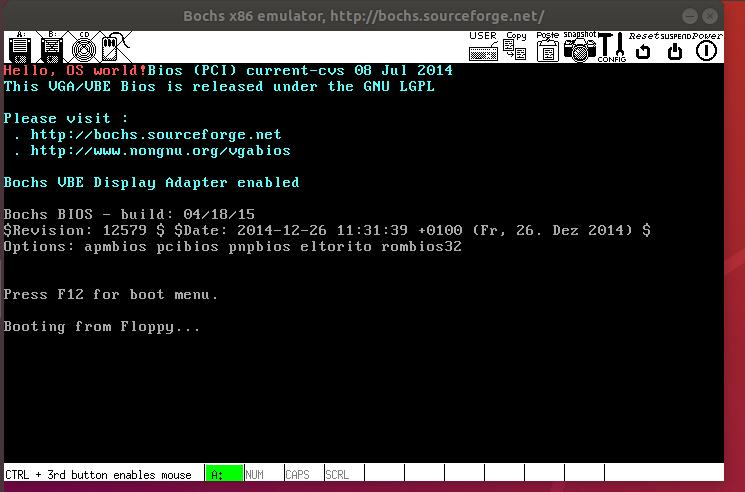
\includegraphics[width=0.8\textwidth]{figures/chapter5/5-1.jpg}
  \caption{引导扇区被DOS识别}
  \label{fig:1}
\end{figure}

这时我们已经为我们的引导扇区加入了 BPB 等头信息,使其可以被DOS识别。接着我们根据实验要求修改boot.asm,使其寻找loader.bin文件。由于我们仅仅是找到Loader.bin就停在那里,这时我们应该使用 Bochs 的调试功能。调试命令如下:
\begin{lstlisting}[language = bash]
  \b ox7c00
  \c
  \n
  \u /45
  \b 0x7cb4
  \c
  \x /32xb es:di -16
  \sreg
  \r
\end{lstlisting}
调试过程如下图 5-2、5-3、5-4 所示:

\begin{figure}[H]
  \centering
  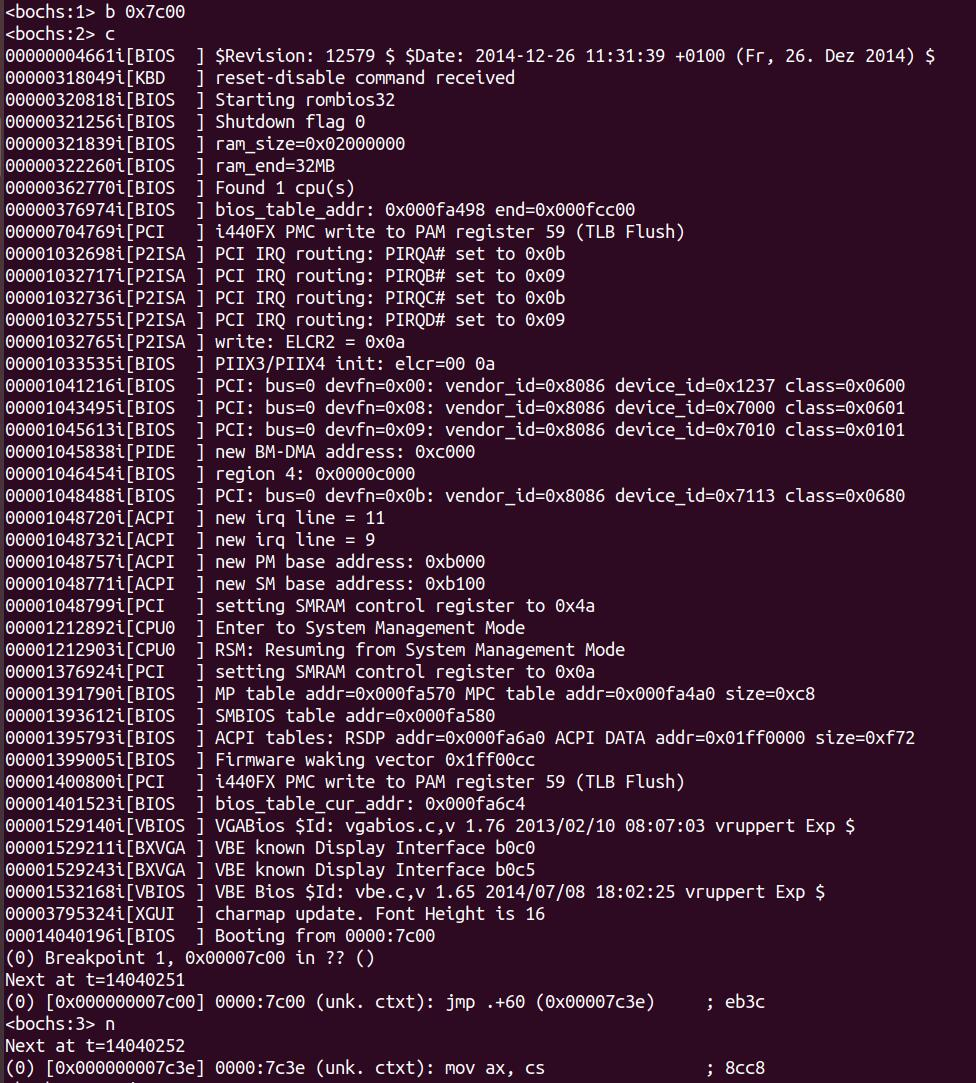
\includegraphics[width=0.8\textwidth]{figures/chapter5/5-2.jpg}
  \caption{调试过程 1}
  \label{fig:2}
\end{figure}

\begin{figure}[H]
  \centering
  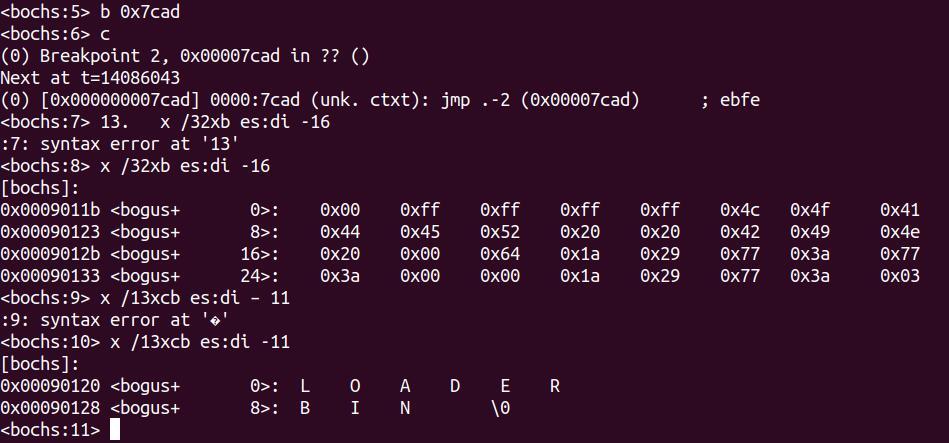
\includegraphics[width=0.8\textwidth]{figures/chapter5/5-3.jpg}
  \caption{调试过程 2}
  \label{fig:3}
\end{figure}

\begin{figure}[H]
  \centering
  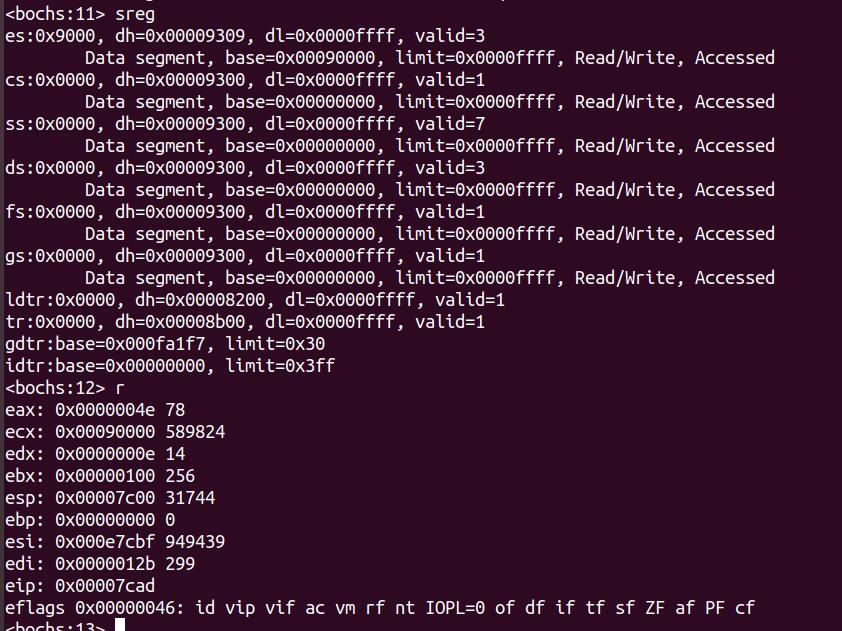
\includegraphics[width=0.8\textwidth]{figures/chapter5/5-4.jpg}
  \caption{调试过程 3}
  \label{fig:4}
\end{figure}

最后,再次修改boot.asm使其将控制权交给loader.bin。调试结果如下图5-5所示:
\begin{figure}[H]
  \centering
  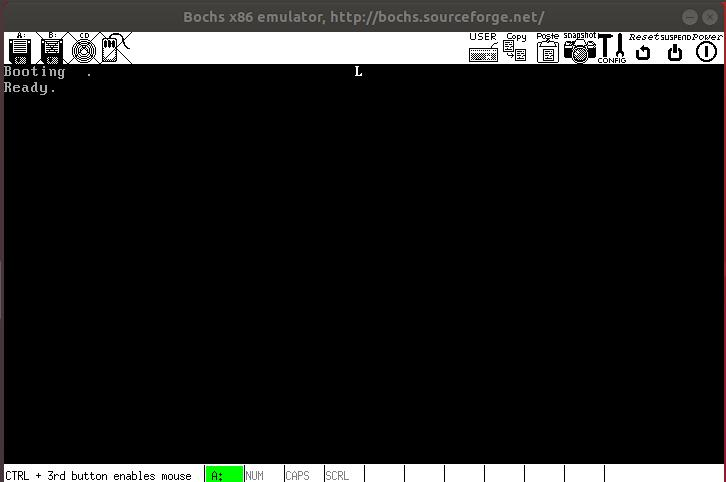
\includegraphics[width=0.8\textwidth]{figures/chapter5/5-5.jpg}
  \caption{控制权交给loader}
  \label{fig:5}
\end{figure}

\section{实验总结}
为突破 512 字节限制,我们进入保护模式的具体过程是:引导->加载内核入内存->跳入保护模式->开始执行内核,这样的工作如果全部交给引导扇区做,空间会不够,因此我们将其交给 Loader 模块完成,引导扇区负责把 Loader 载入内存并将控制权移交给它。我使用的软盘是FAT12 格式。FAT12 格式分为若干个扇区,引导扇区是整个磁盘的第 0 个扇区,在这个扇区中有一个重要数据结构 BPB,说明 FAT 的内容,之后则依次是 FAT1、FAT2、根目录区及数据区。而引导扇区需要有 BPB 等头信息才能被识别,故将其添加在boot.asm开头。\par
在本实验中,我们实现了 boot.asm ,使其可以从软盘中读出 Loader.bin文件,并且加载入内核,同时移交控制权。只要一个.COM 文件中不含有 DOS 系统调用,我们就可以将它当成 Loader 使用,现在的程序已经可以被看做是一个在保护模式下执行的“操作系统”了。但是,我们目前的 Loader 仅仅只是一个 Loader,它不是操作系统内核,也不能当做操作系统内核,操作系统内核应该至少可以在 Linux 下用 GCC 编译链接,摆脱汇编语言,而 Loader 至少要实现两个功能:将内核加载入内存和跳入保护模式。
